%%%%%%%%%%%%%%%%%%%%%%%%%%%%%%%%%%%%%%%%%%%%%%%%%%%%%%%%%%%%%%%%%%%%%%
% LaTeX Template: Beamer arrows
%
% Source: http://www.texample.net/
% Feel free to distribute this template, but please keep the
% referal to TeXample.net.
% Date: Nov 2006
% 
%%%%%%%%%%%%%%%%%%%%%%%%%%%%%%%%%%%%%%%%%%%%%%%%%%%%%%%%%%%%%%%%%%%%%%
% How to use writeLaTeX: 
%
% You edit the source code here on the left, and the preview on the
% right shows you the result within a few seconds.
%
% Bookmark this page and share the URL with your co-authors. They can
% edit at the same time!
%
% You can upload figures, bibliographies, custom classes and
% styles using the files menu.
%
% If you're new to LaTeX, the wikibook is a great place to start:
% http://en.wikibooks.org/wiki/LaTeX
%
%%%%%%%%%%%%%%%%%%%%%%%%%%%%%%%%%%%%%%%%%%%%%%%%%%%%%%%%%%%%%%%%%%%%%%

\documentclass{beamer} %
\usetheme{CambridgeUS}
\usepackage[latin1]{inputenc}
\usefonttheme{professionalfonts}
\usepackage{times}
\usepackage{tikz}
\usepackage{amsmath}
\usepackage{wrapfig}
\usepackage{verbatim}
\usepackage{gensymb}
\usepackage[export]{adjustbox}
\usetikzlibrary{arrows,shapes}

\author{Rachana Yajur}
\title{Design of Beam Diagnostics apparatus for DC Electron Gun}

\begin{document}

\maketitle

\begin{comment}
:Title: Beamer arrows
:Tags: Remember picture, Beamer, Physics & chemistry, Overlays
:Use page: 3

With PGF/TikZ version 1.09 and later, it is possible to draw paths between nodes across
different pictures. This is a useful feature for presentations with the
Beamer package. In this example I've combined the new PGF/TikZ's overlay feature
with Beamer overlays. Download the PDF version to see the result.

**Note.** This only works with PDFTeX, and you have to run PDFTeX twice.

| Author: Kjell Magne Fauske

\end{comment}


% For every picture that defines or uses external nodes, you'll have to
% apply the 'remember picture' style. To avoid some typing, we'll apply
% the style to all pictures.
\tikzstyle{every picture}+=[remember picture]

% By default all math in TikZ nodes are set in inline mode. Change this to
% displaystyle so that we don't get small fractions.
\everymath{\displaystyle}


\begin{frame}{What is my aim?}
    To characterize the electron beams coming from a DC electron gun.  
\end{frame}

\begin{frame}{What are the parameters that needs measurement? }
   
    \begin{enumerate}
    
        \item Longitudinal beam properties
        \begin{itemize}
            \item Beam current
            \item Energy
            \item Energy spread
            \item Bunch size 
            \item Bunch spacing
            \item Charge per bunch
        \end{itemize}
        \item Transverse beam properties
        \begin{itemize}
            \item Emittance ($\epsilon$)
            \item Beam Structure ($\alpha, \beta ,\gamma$)
        \end{itemize}
    \end{enumerate}
    
\end{frame}

\begin{frame}{Electron Gun}
     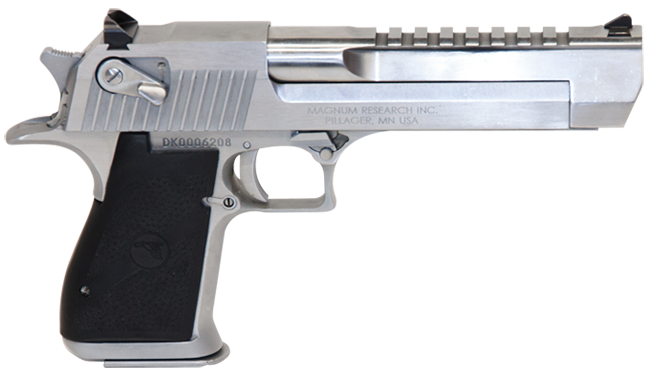
\includegraphics[width=0.1\textwidth]{gun.png}
     \begin{itemize}
        \item DC source with 220V between the cathode and anode
        \item The emittance of the Haimson gun is known to be $10^{-3} \pi mc-cm$
    \end{itemize}

\end{frame}


\begin{frame}{Wall Current Monitor}
    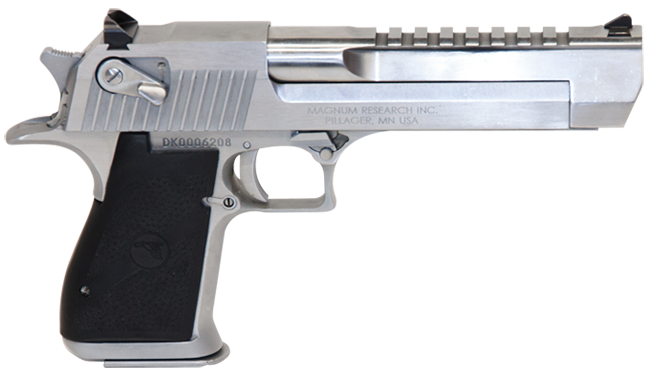
\includegraphics[width=0.1\textwidth]{gun.png}
    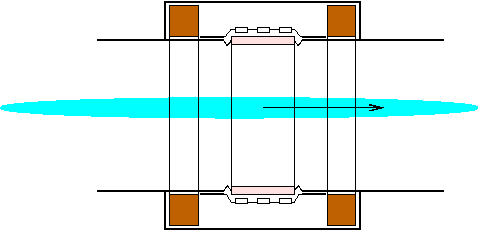
\includegraphics[width=0.2\textwidth]{PSWCM.png}
    \begin{itemize}
        \item Consists of replacing a portion of the vacuum chamber tube with a ceramic ring and measuring the mirror currents across a resistor. 
    \end{itemize}
\end{frame}

\begin{frame}{Quadrupole Scan Technique}
    This is a very strong method to measure the transverse emittance. 
    \begin{figure}
        \centering
         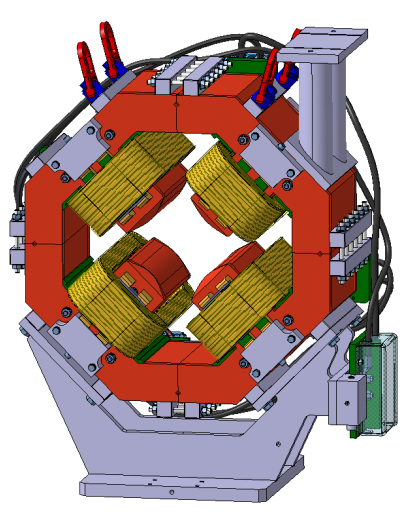
\includegraphics[width=0.1\textwidth]{quad.jpg}
    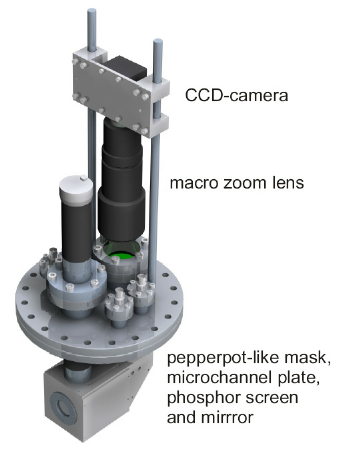
\includegraphics[width=0.15\textwidth]{pepperpot.png}
    \end{figure}
  
    The beam transverse phase space ellipse can be described in terms of a matrix $\sigma(z)$,
    \begin{equation}
        \sigma(z) = \begin{bmatrix} \sigma_{11}&\sigma_{12}\\ \sigma_{21}&\sigma_{22} \end{bmatrix} = \epsilon  \begin{bmatrix}\beta & -\alpha\\ -\alpha & \gamma \end{bmatrix}
    \end{equation}
    \end{frame}
    \begin{frame}{Quadrupole scan technique}
    Let the transfer matrix due to quadrupole be $R = \begin{bmatrix} R_{11}&R_{12}\\ R_{21}&R_{22} \end{bmatrix} $
    Now the $\sigma$ matrix transforms as:
    \begin{equation}
        \sigma(z') = R \sigma(z_0) R^T
    \end{equation}
    If we knew $\sigma_{11}(z')$, then elements of $\sigma(z_0)$ can be expressed as:
    
    \begin{equation}
        \sigma_{11}(z') = R_{11}^2 \sigma_{11} - 2 R_{11}R_{12} \sigma_{12} + R_{12}^2 \sigma_{22} 
     \end{equation}
    Now we can take the measurements for atleast 3 different Q-pole strengths so that we have 3 equations which can solve for the 3 variables.  
\end{frame}

\begin{frame}{Pepper Pot}
    This consists of a metallic grid followed by a fluorescence screen which is followed by a $45\degree$ mirror whose reflection is captured by a CCD camera. With this output we can deduce the transverse beam distribution. Which basically gives us $\sigma_{11}$ along the x and y direction. 
    \begin{figure}
    \centering
     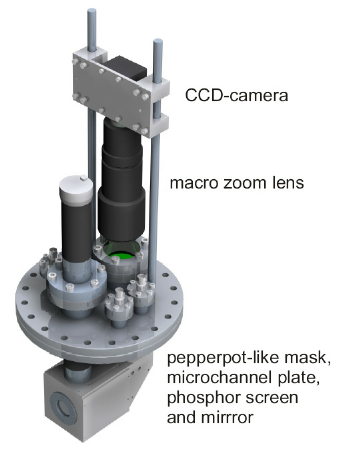
\includegraphics[width=0.25\textwidth]{pepperpot.png}
     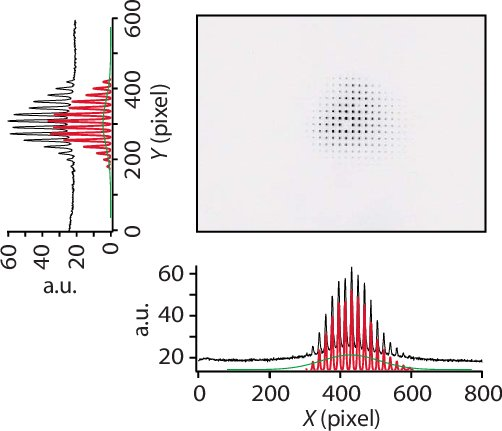
\includegraphics[width=0.35\textwidth]{pepperpotresult.jpg}
     \end{figure}
\end{frame}

\begin{frame}{Dipole Spectrometer}
    A bending dipole can be used to measure the energy of the beam as well as the energy spread by measuring the angular deviation from the original path.  This could be measured by either placing another pepperpot at the expected angle of deviation or have a faraday cup preceded by a bellow so as to allow for movement of the faraday cup which can measure the angular distribution of the beam current, from which energy and energy spread can be calcualted. 
    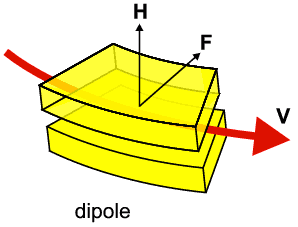
\includegraphics[width=0.2\textwidth]{dipole.png}
    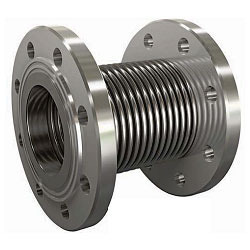
\includegraphics[width=0.1\textwidth]{ss-metallic-expansion-joint-250x250.jpg}
    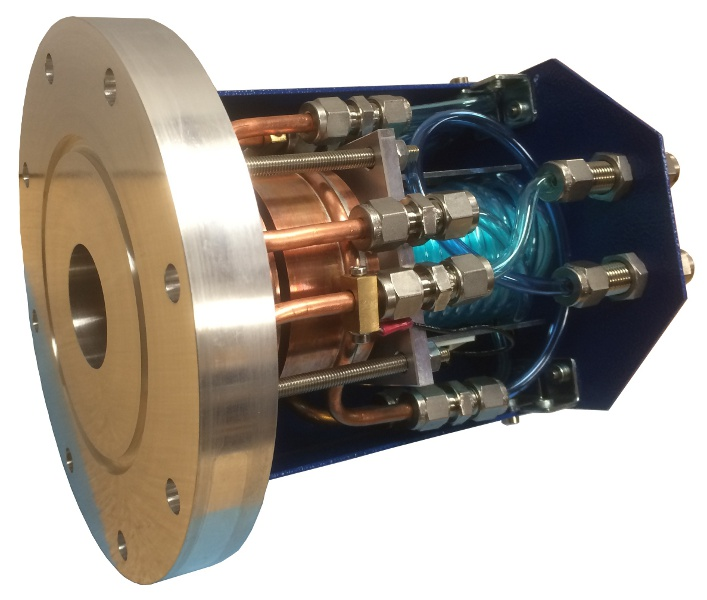
\includegraphics[width=0.15\textwidth]{faraday.JPG}
\end{frame}

\begin{frame}{Story so far}
    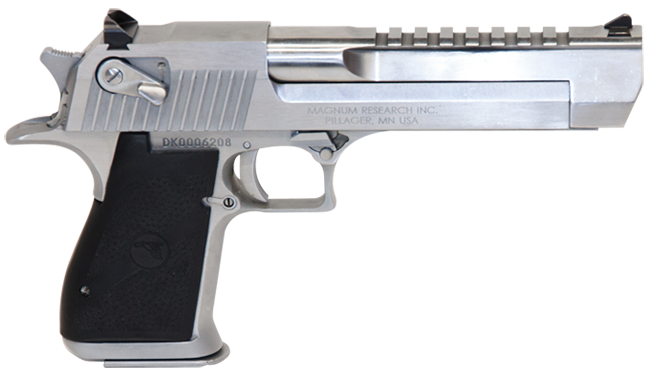
\includegraphics[width=0.1\textwidth]{gun.png}
    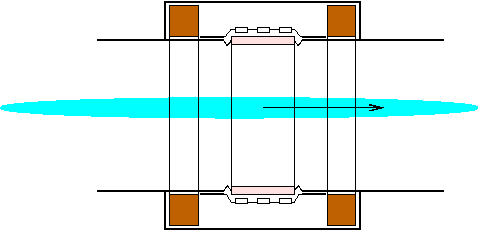
\includegraphics[width=0.2\textwidth]{PSWCM.png}
    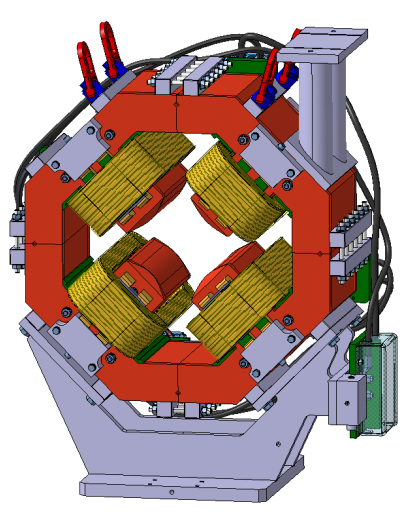
\includegraphics[width=0.1\textwidth]{quad.jpg}
    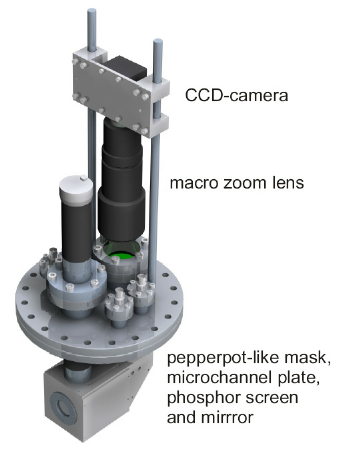
\includegraphics[width=0.15\textwidth]{pepperpot.png}
    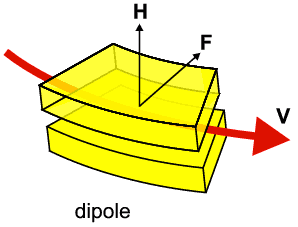
\includegraphics[width=0.2\textwidth]{dipole.png}
    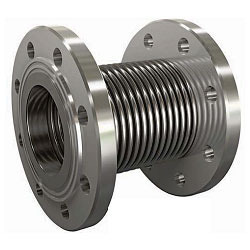
\includegraphics[width=0.1\textwidth]{ss-metallic-expansion-joint-250x250.jpg}
    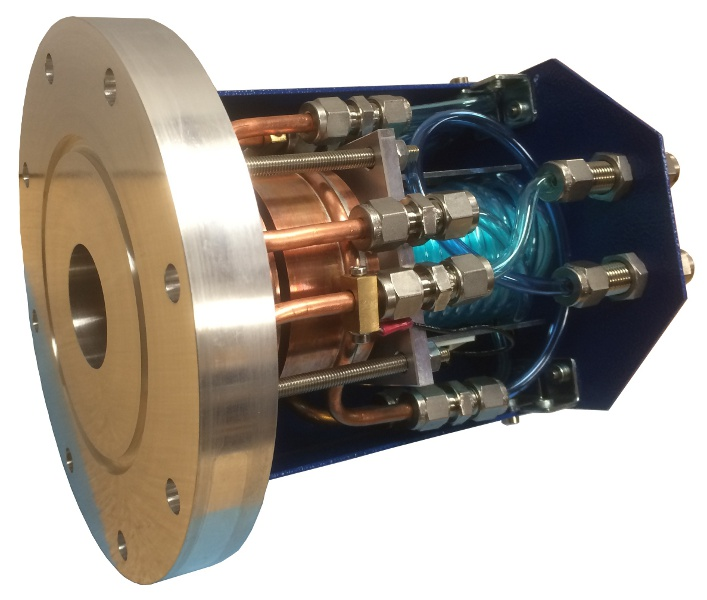
\includegraphics[width=0.15\textwidth]{faraday.JPG}
\end{frame}




\begin{frame}{Problems}
    \begin{itemize}
        \item Should beam current transformer, beam position monitors, solenoids or any other diagnostic device be necessarily used? 
        \item Are there any redundancies in the current design?
        \item How to quantify the reliability of the current design? 
        \item What are the constraints and limitations that needs to be considered?
    \end{itemize}
\end{frame}



\begin{frame}{Future Work}
    \begin{itemize}
        \item Simulate the diagnostic apparatus in CST Studio/Astra for different configurations to converge on an optimal design.  
        \item Decide the optimum parameters required for the quadrupole and dipole construction.
        \item Decide the size and shape of the apparatus
    \end{itemize}
\end{frame}

\begin{frame}{}
\centering
Thank you
    
\end{frame}


\begin{comment}


\begin{frame}
\frametitle{Rigid body dynamics}

\tikzstyle{na} = [baseline=-.5ex]

\begin{itemize}[<+-| alert@+>]
    \item Coriolis acceleration
        \tikz[na] \node[coordinate] (n1) {};
\end{itemize}

% Below we mix an ordinary equation with TikZ nodes. Note that we have to
% adjust the baseline of the nodes to get proper alignment with the rest of
% the equation.
\begin{equation*}
\vec{a}_p = \vec{a}_o+\frac{{}^bd^2}{dt^2}\vec{r} +
        \tikz[baseline]{
            \node[fill=blue!20,anchor=base] (t1)
            {$ 2\vec{\omega}_{ib}\times\frac{{}^bd}{dt}\vec{r}$};
        } +
        \tikz[baseline]{
            \node[fill=red!20, ellipse,anchor=base] (t2)
            {$\vec{\alpha}_{ib}\times\vec{r}$};
        } +
        \tikz[baseline]{
            \node[fill=green!20,anchor=base] (t3)
            {$\vec{\omega}_{ib}\times(\vec{\omega}_{ib}\times\vec{r})$};
        }
\end{equation*}

\begin{itemize}[<+-| alert@+>]
    \item Transversal acceleration
        \tikz[na]\node [coordinate] (n2) {};
    \item Centripetal acceleration
        \tikz[na]\node [coordinate] (n3) {};
\end{itemize}

% Now it's time to draw some edges between the global nodes. Note that we
% have to apply the 'overlay' style.
\begin{tikzpicture}[overlay]
        \path[->]<1-> (n1) edge [bend left] (t1);
        \path[->]<2-> (n2) edge [bend right] (t2);
        \path[->]<3-> (n3) edge [out=0, in=-90] (t3);
\end{tikzpicture}
\end{frame}

\end{comment}

\end{document}